\documentclass[a4paper,fleqn]{article}
\usepackage{ngerman,graphicx,amsmath,amssymb,mathbbol}
\usepackage[utf8]{inputenc}

\usepackage{tikz}
\usetikzlibrary{external}
\tikzexternalize
\tikzsetexternalprefix{figure_}
\tikzset{external/mode=list and make}
\tikzset{external/export=true}

\begin{document}

% First: normale figure
\begin{center}
  
\begin{tikzpicture}
    \node[draw,circle]{A};
  \end{tikzpicture}
\end{center}

% Second: a non-externalised figure
\begin{center}
  \tikzset{external/export=false}
  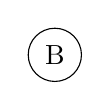
\begin{tikzpicture}
    \node[draw,circle]{B};
  \end{tikzpicture}
  \tikzset{external/export=true}
\end{center}

% Third: externalise again with custom name
\begin{center}
  \tikzsetnextfilename{thirdtest}
  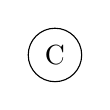
\begin{tikzpicture}
    \node[draw,circle]{C};
  \end{tikzpicture}
\end{center}

% Fourth: figure with errors
\begin{center}
  \tikzsetnextfilename{errortest}
  \begin{tikzpicture}[]
    \node[draw,circle]{\Rightarrow}
    \path (a) -- ;
  \end{tikzpicture}
\end{center}

\end{document}
